% !TEX root = ../thesis.tex

\chapter{Numerical Simulations} \label{ch:experiments}
In this chapter, we start by discussing two practical aspects related to the experimental applications of the algorithms described in Chapter (\ref{ch:core}). Then, we proceed by showing the results of our numerical simulations on three \gls{RL} benchmarking challenges: the \gls{LQG}, the Continuous Mountain Car problem and the Inverted Pendulum task.

The programming language chosen for implementing the numerical simulations discussed in this chapter is Python. The code is publicly available on GitHub\footnote{https://github.com/T3p/baselines/tree/exploration/baselines}, and it is built upon the OpenAI Baselines library\footnote{https://github.com/openai/baselines}.

\section{Practical Aspects} \label{sec:practical}
In the numerical simulations that will be presented in the following sections we place ourselves in the \emph{parameter-based} \gls{PS} setting (see Section (\ref{sec:problem}) for details). We adopt Gaussian distributions as target and behavioural hyperpolicies $\nu_{\vxi}= \mathcal{N}(\vmu,\Cov)$, from which the policy parameters $\vtheta$ are drawn. In particular, we will adopt diagonal hyperpolicies $\nu_{\vxi}$, with hyperparameters $\vxi=\{\vtheta,\Cov\}$, of the form: 

\begin{align}
\nu_{\vxi}(\vtheta) & = \frac{1}{\sqrt{(2\pi)^m |\Cov |}}\exp\left(
	-\frac{1}{2} (\vtheta - \vmu )^T\Cov^{-1}(\vtheta - \vmu )\right)\\
	& = \frac{1}{\sqrt{(2\pi)^m \prod_{i=1}^{m} \sigmai^2}}\exp\left(
	-\frac{1}{2} \sum\limits_{i=1}^m\frac{(\thetai-\mui)^2}{\sigmai^2}\right).
\end{align}

This allows the use of a deterministic controller $\pi_{\vtheta}: \vtheta\in\Theta\subseteq\Reals^m$ for sampling the trajectories, that we define as $\pi_{\vtheta}(a|s)=\delta(a-\vtheta s)$. This parameter-based setting follows the one adopted in \gls{PGPE}, as described in (\ref{subsec:algorithms}). \\
This distribution choice for our target and behavioural hyperpolicies allows a comfortable computation of the robust balance heuristic estimator $\wc{\mu}_t(\vx)$ defined in Equation (\ref{eq:wcmu}). Unfortunately, that is not all for the computation of the upper bound $B_t^{\epsilon}(\vx,\delta_t)$ (\ref{eq:optimistindex}) that we need to optimize in each iteration $t$ of \gls{OPTIMIST}.

\subsection{Divergence Between Gaussian Multivariate Distributions}

Indeed, \gls{OPTIMIST} also requires to compute the exponentiated \Renyi divergence between the target hyperpolicy $p_{\vx}$ 
and the mixture $\Phi_t$, \ie $d_{1+\epsilon}(p_{\vx}\|\Phi_t)=d_{1+\epsilon}(\nu_{\vxi}\|\Phi_t)$, at each iteration. Even for Gaussian distributions, this quantity cannot be obtained in closed form, while
the \Renyi divergence between Gaussians can be computed exactly. In this section, we provide an upper bound for computing the exponentiated \Renyi divergence
between a generic distribution and a mixture.
\begin{restatable}{theorem}{armonic}\label{th:armonic}
	Let $P$ be a probability measure and $\Phi = \sum_{k=1}^K \beta_k Q_k$, with $\beta_k \in [0,1]$ and $\sum_{k=1}^K \beta_k =1$, be a finite mixture of the
	probability measures $\{Q_k\}_{k=1}^K$. Then, for any $\alpha \ge 1$, the exponentiated $\alpha$-\Renyi divergence can be bounded as: 
	\begin{equation}
	d_{\alpha}(P \| \Phi) \le \frac{1} {\sum_{k=1}^K \frac{ \beta_k}{ d_{\alpha}(P \| Q_k)}}.
	\end{equation}
\end{restatable}

The proof can be found in Appendix~\ref{app:proof}. We can easily compute this upper bound of the exponentiated \Renyi divergence between the target distribution and the mixture of behavioural distributions. In fact, all the hyperpolicies employed are multivariate diagonal Gaussian distributions, and the \Renyi divergence between multivariate Gaussian distributions is known \cite{gil2013renyi}. Let $P\sim\mathcal{N}(\vmu_P,\Cov_P)$, $Q\sim\mathcal{N}(\vmu_Q,\Cov_Q)$ and $\alpha\in[0,\infty]$:

\begin{align} \label{eq:gaussianrenyi}
D_{\alpha}(P||Q) &= \frac{1}{\alpha}(\vmu_P-\vmu_Q)^T\Cov_\alpha^{-1}(\vmu_P-\vmu_Q)-\frac{1}{2(\alpha-1)}\log\frac{\det(\Cov_{\alpha})}{\det(\Cov_P)^{1-\alpha}\det(\Cov_Q)^{\alpha}},
\end{align}

where $\Cov_{\alpha}=\alpha\Cov_Q+(1-\alpha)\Cov_P$ under the assumption that $\Cov_{\alpha}$ is positive-definite.

\subsection{Uniformly Bounded Rényi divergence} \label{subsec:boundrenyi}

The other concern about the exponentiated \Renyi divergence between the target and the mixture of behavioural hyperpolicies is to make it compliant with Assumption (\ref{ass:boundrenyi}), \ie to make it uniformly bounded. Without this assumption, the results on \gls{OPTIMIST} regret (Theorems (\ref{th:regretdiscrete}),(\ref{th:regretcompact}) and (\ref{th:regretdiscretized})) are no more guaranteed. This assumption can be easily respected by careful hyperpolicy design. First, note that the results on the regret are provided for a compact continuous (or finite discrete) arm set, hence the maximum distance among the parameters is bounded. Additionally, we must ensure that the \Renyi divergence is bounded. As showed in Theorem (\ref{th:armonic}), it is enough that the divergence is finite between the target and one of the components of the mixture to guarantee a bound on the divergence between a target distribution and a mixture of behavioural distributions. Hence, we will focus on the constraints between behavioural/target pairs. As an example, for multivariate diagonal Gaussian distributions with fixed covariance Assumption (\ref{ass:boundrenyi}) is easily guaranteed. In fact, the \Renyi divergence is a continuous function of the mean parameter \cite{gil2013renyi} and a continuous function on a compact set is bounded. If the standard deviation (or covariance matrix) is also part of the parameter set, additional constraints are needed, as one can understand by examining Equation (\ref{eq:gaussianrenyi}). For $\epsilon=1$, the standard deviation $\sigma_P$ of the target distribution must not be larger than twice that of the behavioural ($\sigma_Q$) for the divergence to be finite. Hence, given a minimum $\sigma_{0} > 0$, it is enough to constrain the search within $[\sigma_0, 2*\sigma_0]$. We also suggest initializing the first behavioural distribution with $\sigma_Q=2*\sigma_0$, so that the algorithm will move towards smaller standard deviations. This will result in a less stochastic behaviour. Similar constraints can be defined for other kinds of policies \cite{gil2013renyi}. 


\section{Linear Quadratic Gaussian Regulator}
The goal of our numerical simulations on \gls{LQG} is twofold. First, we need a simple continuous control problem to understand the functioning of our algorithms. Second, we want to compare \gls{OPTIMIST} (Algorithm (\ref{alg:1})) with two classical \gls{MAB} algorithms presented in Chapter (\ref{ch:sota}): \gls{UCB}1 (\ref{sebsec:count&UCB}) and \gls{GPUCB} (\ref{alg:gpucb}), in the case of discrete parameter space $\Xi$.\\
The \gls{LQG} problem \cite{peters2008reinforcement} is a continuous \gls{MDP} which represents a useful testing ground for control algorithms, mainly because of its simplicity. At each time-step $h$, the transition kernel and reward function are given by:

\begin{align}
\boldsymbol{s}_{h+1}=\boldsymbol{A}\boldsymbol{s}_h+\boldsymbol{B}\boldsymbol{a}_h +\boldsymbol{\eta}_h\\
r_h=\boldsymbol{s}_{h}^T\boldsymbol{Q}\boldsymbol{s}_{h}+\boldsymbol{a}_{h}^T\boldsymbol{R}\boldsymbol{a}_{h}
\end{align}

where $\boldsymbol{A}$, $\boldsymbol{B}$, $\boldsymbol{Q}$ and $\boldsymbol{R}$ are coefficient matrices and $\boldsymbol{\eta}_h$ is a noise process assumed to be a Gaussian white noise $\boldsymbol{\eta}_h\sim\mathcal{N}(\boldsymbol{0}, \Cov_{LQG})$ with uncorrelated components $\Cov_{LQG}=\sigma_{LQG}\boldsymbol{I}$. The reward $r_h$ has to be intended as a cost for the agent, something it wants to avoid.
Intuitively, in this problem the agent has to bring its state to zero, while facing a cost proportional to the magnitude of its state and action. The optimal control policy in steady state conditions is the linear controller $\boldsymbol{a}_{h}=\boldsymbol{K}\boldsymbol{s}_{h}$, where matrix $\boldsymbol{K}$ can be found by solving a Riccati equation \cite{dorato1995linear}. We conducted our experiments on one-dimensional \gls{LQG}. 
For implementation reasons, we consider the case in which the state space is limited to $\Sspace=[-4,4]$, the action space is $\Aspace=[-4,4]$ and the horizon is limited to $H=20$. At the beginning of the episode, the start-state is initialized randomly $s_0\sim\mathcal{U}([-4,4])$. The agent samples $H=20$ steps-long trajectories with a discount factor of $\gamma=0.99$, for a total of $T=5000$ iterations.

As mentioned in the previous section, in all our experiments we employ diagonal Gaussian hyperpolicies. In this case the hyperpolicy is univariate $\nu_{\vxi} = \mathcal{N}(\mu, \sigma^2)$, where $\mu$ is the mean parameter to be learned and $\sigma$ can be either fixed or learnable as well. On the other hand, the policy $\pi_{\theta}$ adopted by the agent is a deterministic linear controller $a_h=\pi_{\theta}(s_h)=\theta\cdot s_h$, with $\theta\sim\nu_{\vxi}$. Since \gls{UCB}1 requires a positive return $r_t\in[0,1]$, we standardized the trajectory return $\Rew(\vxi_t)=\sum_{h=0}^{H-1}\gamma^h r_{h+1}$ associated to the arm $\xi_t$ pulled at iteration $t$: 

\begin{align}
r_t=\Rew(\vxi_t)/\Rew(\vxi^*),
\end{align}

where $\vxi^*$ is the optimal arm and $\Rew(\vxi^*)$ is the maximum achievable cumulated return:

\begin{align}
\Rew(\vxi^*)
&= \sum_{h=0}^{H-1}\gamma^h\cdot 1 = \frac{1-\gamma^h}{1-\gamma}.
\end{align}
 
Each of these  All algorithms are run with the confidence schedule proposed in Theorem (\ref{th:regretdiscrete}), \ie $\delta_t = \frac{3\delta}{t^2\pi^2K}$, with $\delta=0.2$ (similar results have been obtained with different values of $\delta$). The parameters used in the \gls{LQG} experiments are summarized in Table (\ref{tab:LQGcoeff}).


\begin{table}[t!]
\centering
\begin{tabular}{cccc|cccc|c} 
\toprule
a & b & q & r & $\gamma$ & H & T & $\sigma_{LQG}$ & $\delta$\\ 
\midrule
1.00 & 1.00 & 0.90 & 0.90 & 0.99 & 20 & 5000 & 0.10 & 0.20\\
\bottomrule
\end{tabular}
\caption{Environmental coefficients (left-side), task coefficients (center) and \gls{OPTIMIST} input parameters (right-side) for the \gls{LQG} experiments.}
\label{tab:LQGcoeff}
\end{table}


\subsection{Gain only}

\begin{figure}[t!]
\centering
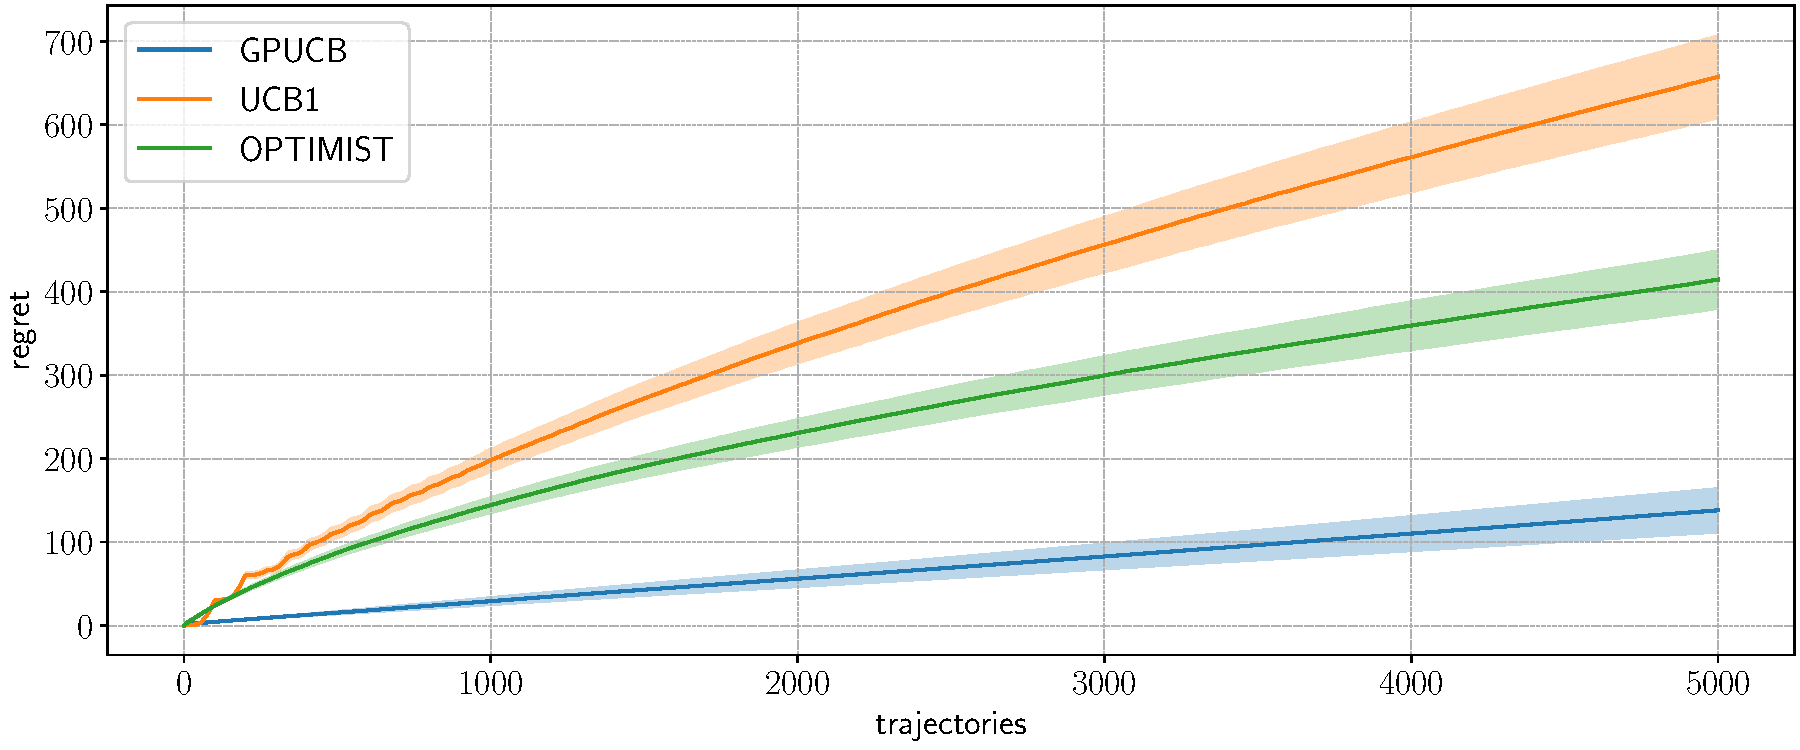
\includegraphics[width=\textwidth,height=\textheight,keepaspectratio]{Images/LQGcomparison.pdf}
\caption{Cumulative regret in
the \gls{LQG} experiment. Comparison between
\gls{OPTIMIST}, \gls{UCB}1 and \gls{GPUCB} when learning the hyperpolicy mean.
(30 runs, 95\% c.i.)}
\label{fig:LQGcomparison}
\end{figure}

\begin{figure*}[t!] 
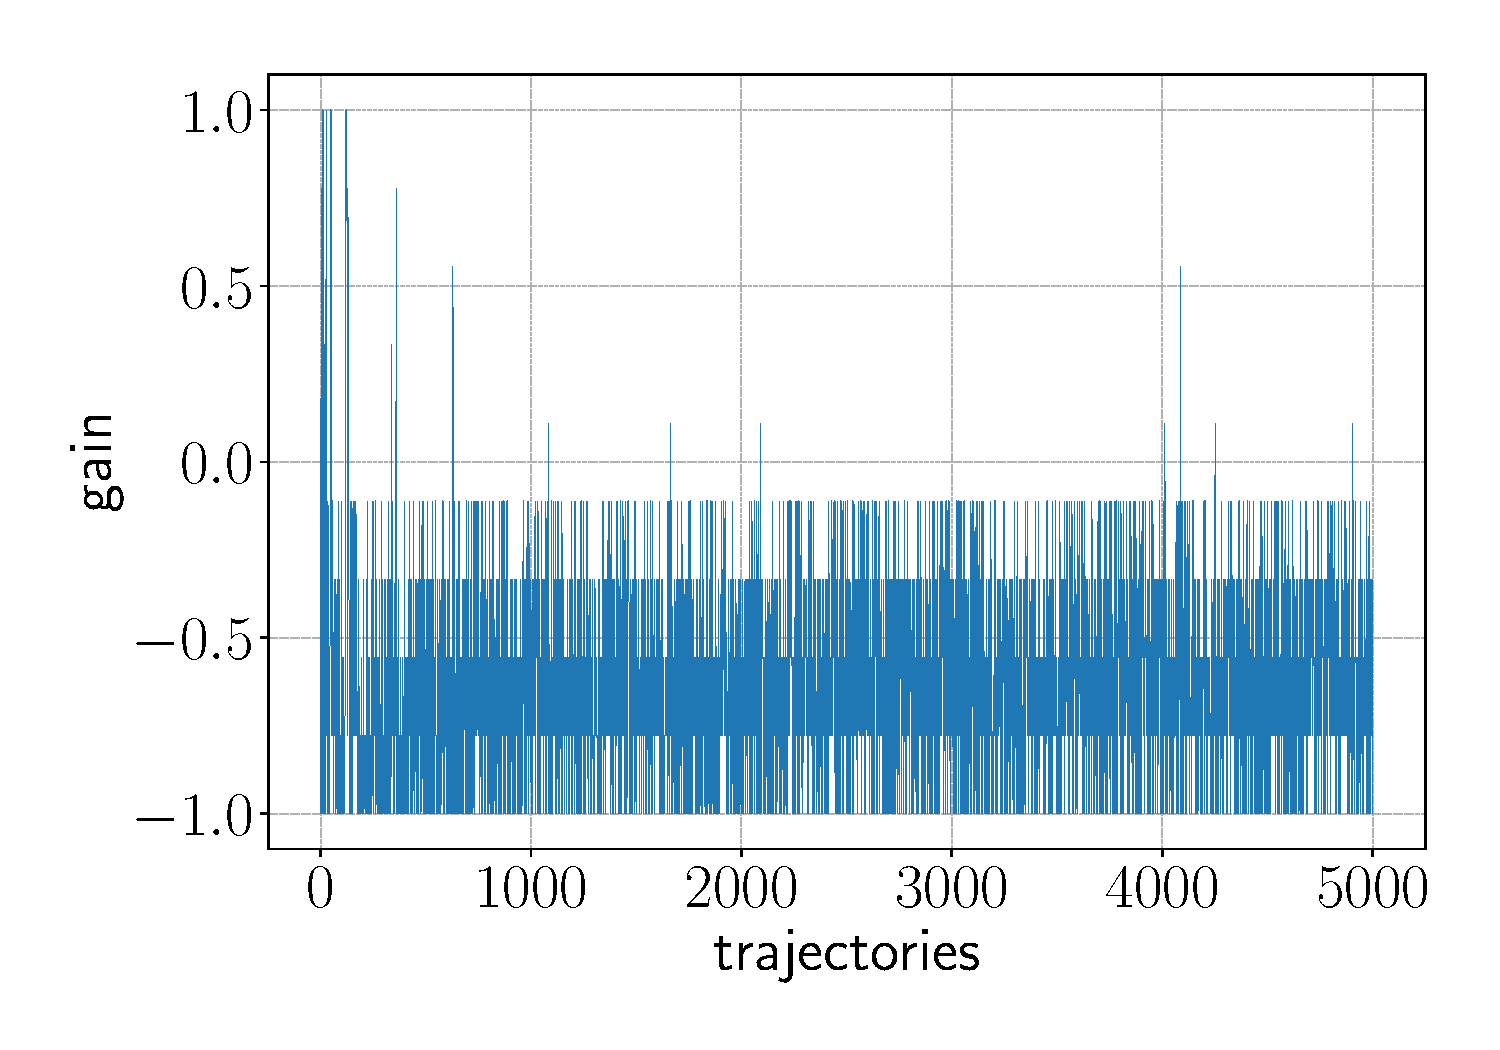
\includegraphics[width=.5\textwidth]{Images/LQG_GPUCB_mu.pdf}\hfill
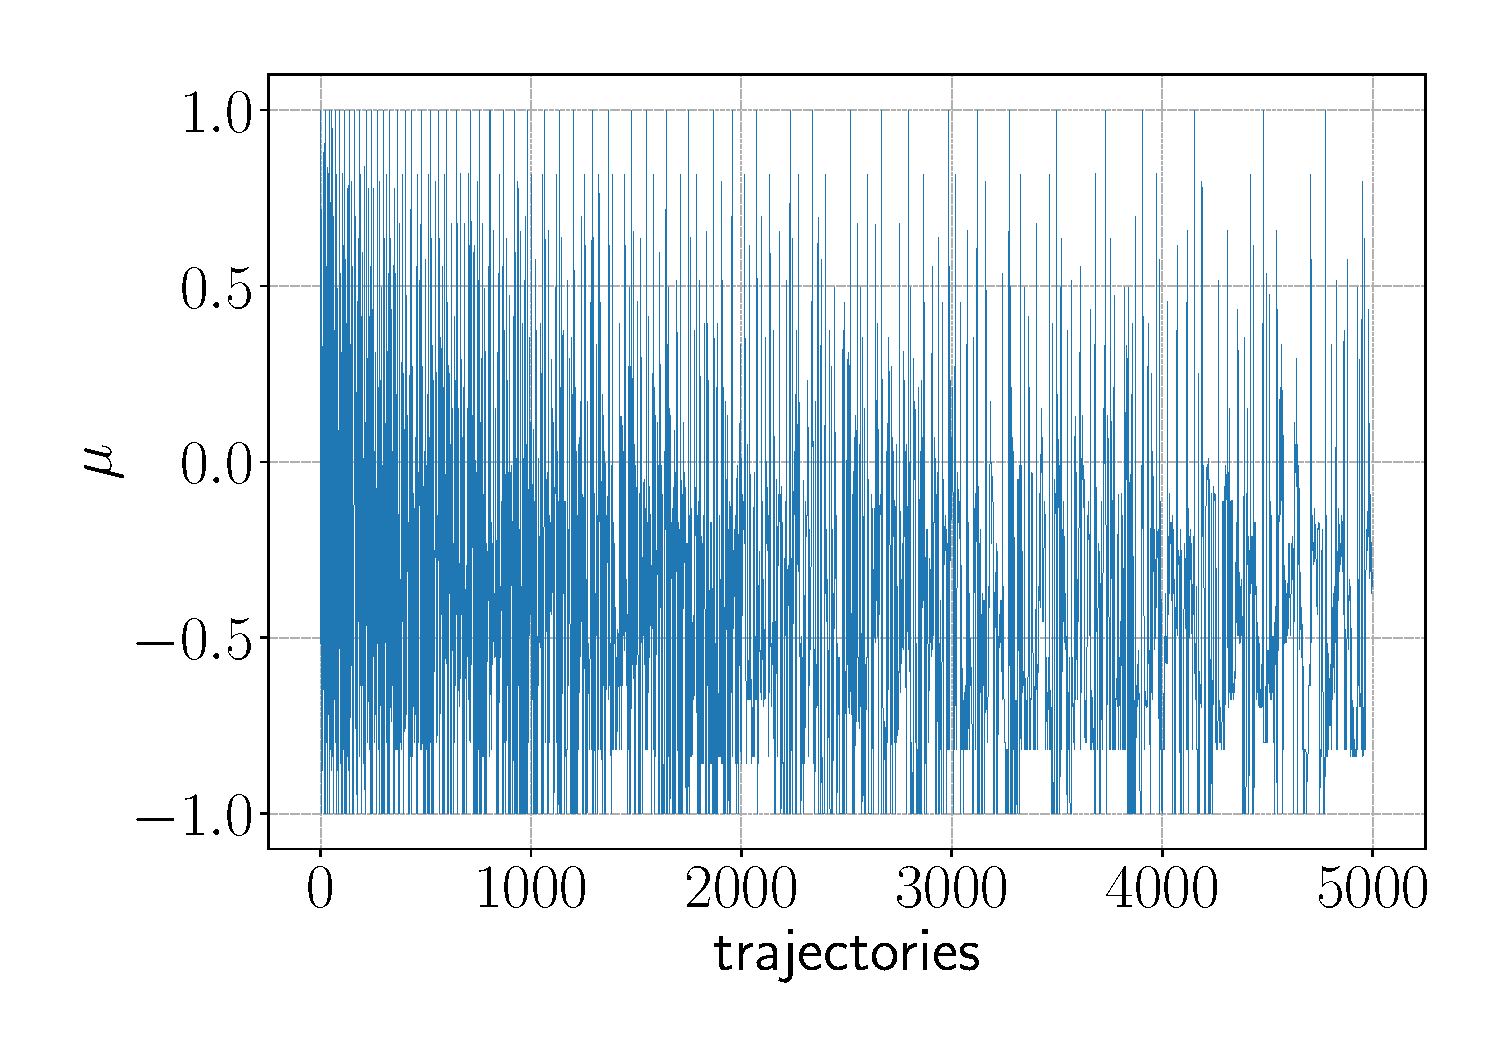
\includegraphics[width=.5\textwidth]{Images/LQG_OPTIMIST_mu.pdf}\hfill
%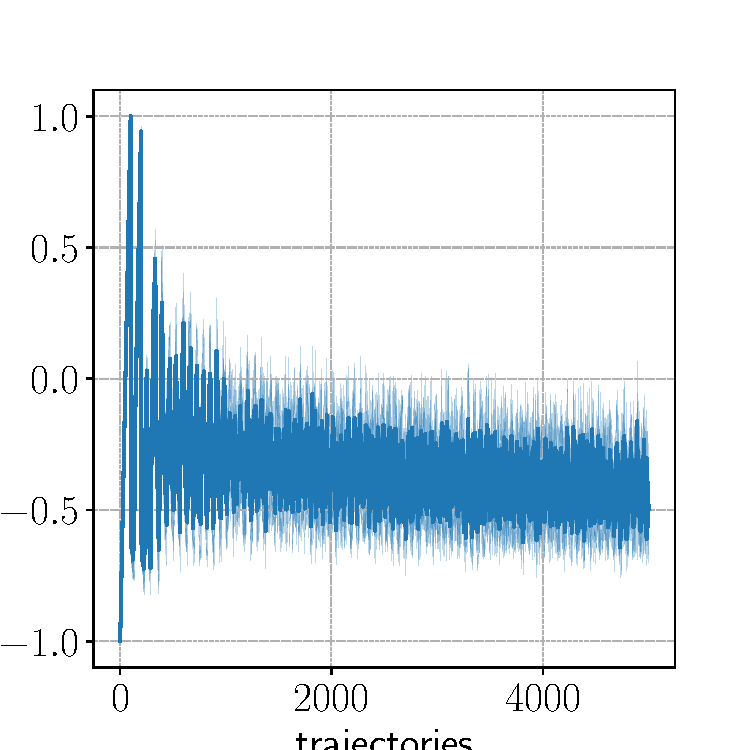
\includegraphics[width=.33\textwidth]{Images/LQG_UCB1_mu.pdf}
\caption{The gain parameter $\mu$ selected at each iteration of \gls{GPUCB} (left) and \gls{OPTIMIST} (right) in the \gls{LQG} experiment.}
\label{fig:LQGmu}
\end{figure*}


\begin{figure}[t!]
\centering
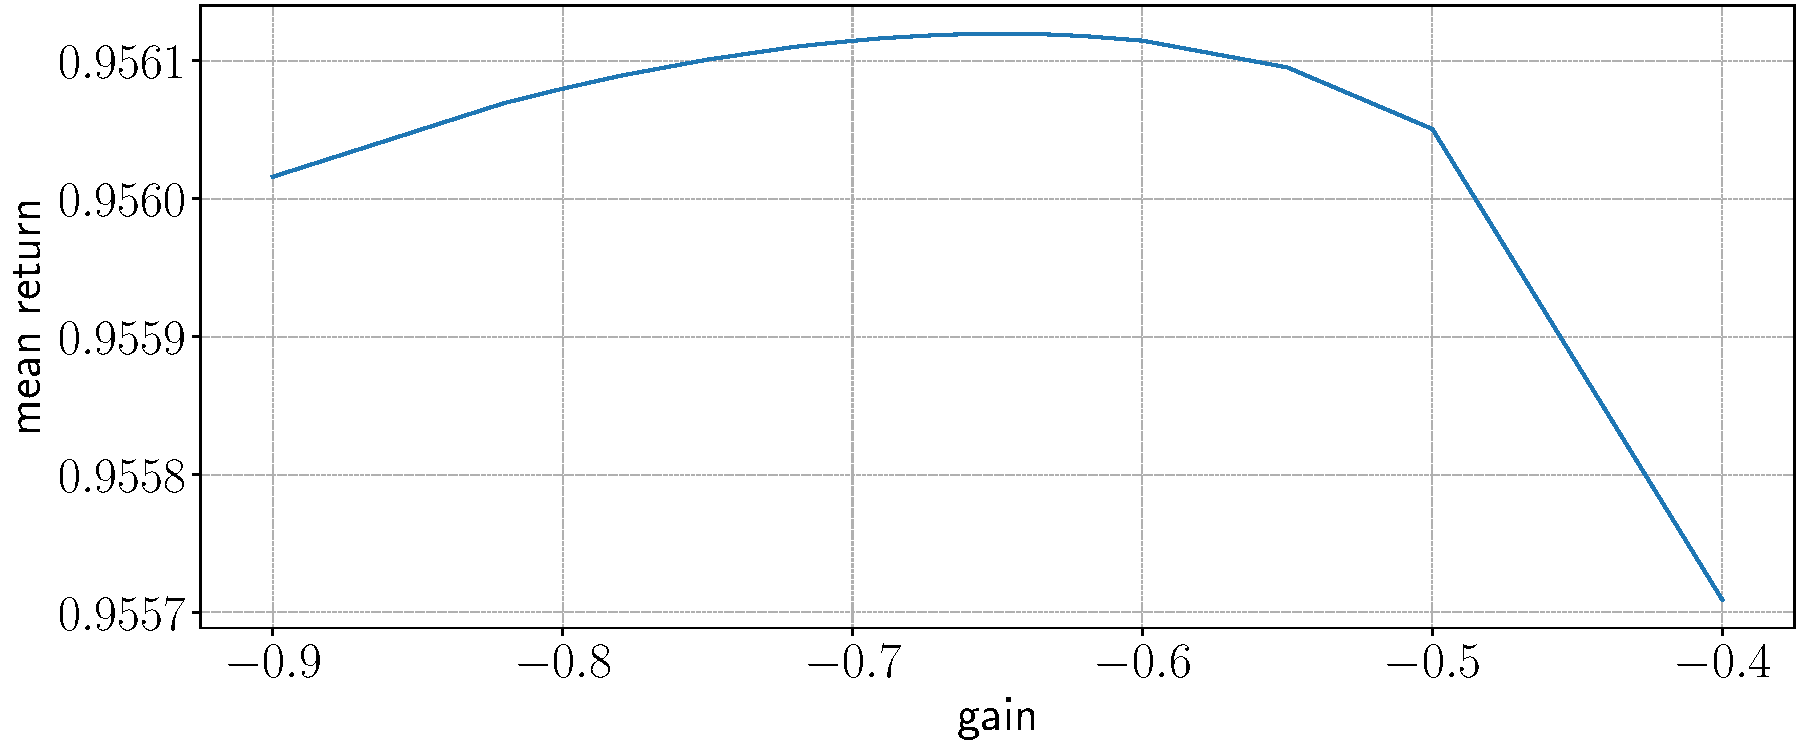
\includegraphics[width=.75\textwidth,keepaspectratio]{Images/LQG_optimal_gain.pdf}
\caption{Mean return of arms $\mu\in[-0.9,-0,5]$, calculated by averaging the return collected over 2000 trajectories in the \gls{LQG} experiment.}
\label{fig:LQGoptimalgain}
\end{figure}

In order to benchmark \gls{OPTIMIST} with both \gls{UCB}1 and \gls{GPUCB} on a discrete set, we first consider the case in which the only learnable parameter of $\nu_{\vxi}$ is the gain $\mu$. To this end, we consider a uniform discretization of the interval $[-1,1]$ made of 100 arms (every arm is a possible choice of $\mu$). The hyperpolicy standard deviation is fixed to $\sigma=0.15$. We experimented with different values of $\sigma$ and this turned out to be a good choice for making the task noisy, but not too noisy to allow learning.


In Figure (\ref{fig:LQGcomparison}), we show the cumulative regret of the three algorithms, averaged over 30 runs. We can see that our algorithm significantly outperforms \gls{UCB}1.
Indeed, \gls{OPTIMIST} is able to exploit the structure of arms, \ie hyperpolicies, by means of the \gls{MIS} estimation, whereas \gls{UCB}1 does not make any assumption on arm correlation. In other words, \gls{OPTIMIST} performs a more informed (directed) exploration, leveraging what the agent has experienced in past episodes more effectively. On the contrary, \gls{GPUCB} shows a better performance \wrt to \gls{OPTIMIST}. We point out that \gls{GPUCB} requires to specify, at the beginning of learning, the kernel of the Gaussian process from which the payoff function is sampled. We employed the default scikit-learn\footnote{A popular library for data mining and data analysis. Available at: https://scikit-learn.org/stable/} kernel, \ie the radial basis function kernel:

\begin{align}
	k_T(\vx,\vx') &= \exp\left(-\lambda\norm{\vx-\vx'}^2\right),
\end{align}

where $\lambda$ is a free parameter. However, as it often happens in control tasks, our payoff is not actually sampled from a Gaussian process. This invalidates all theoretical guarantees of \gls{GPUCB} and may be at the root of its strong commitment to exploitation, contrary to \gls{UCB}1 and \gls{OPTIMIST}. We can visualize the amount of exploration carried out by the three algorithms by looking at Figure (\ref{fig:LQGmu}), which depicts, the arm $\mu$ pulled by \gls{GPUCB} and \gls{OPTIMIST} at every iteration. Indeed, \gls{OPTIMIST} explores the set of arms around the optimum much more extensively then \gls{GPUCB}, which, in the very first steps, commits to a near-optimal set of arms (the neighbourhood of $\mu=-0.5$ interval) and sticks to it all along. This explains the lower regret of \gls{GPUCB} \wrt \gls{OPTIMIST}. In fact, the \gls{LQG} task presents a pretty wide set of optimal or near-optimal arms spanning in $[-0.9,-0.5]$, as shown in Figure (\ref{fig:LQGoptimalgain}). Therefore, exploitation is a rewarding strategy in this setting.


\subsection{Gain and standard deviation}
In the second experiment on \gls{LQG}, we learn both the mean and the variance parameter of the Gaussian hyperpolicy: $\nu_{\vxi} = \mathcal{N}(\mu, \exp(2\sigma))$, where $\vxi=(\mu,\sigma)^T=(\xi_1,\xi_2)^T$. The parameters used in the experiment are the same as before, reported in Table (\ref{tab:LQGcoeff}).
In Figure (\ref{fig:LQGcomparisonVar}), we show the cumulative regret averaged over 5 runs comparing \gls{OPTIMIST}, \gls{UCB}1 and \gls{GPUCB}. We see a trend similar to the case in which we learn only the mean parameter. While \gls{OPTIMIST} is able to exploit the structure of the arms induced by the fact that hyperpolicies share information, beating \gls{UCB}1, \gls{GPUCB} still displays a better performance. The wider confidence intervals are a direct consequence of the wider spectrum of variances adopted by the hyperpolicy, bringing to very different choices of policy parameters and, subsequently, very difference performance from one run to another.

\begin{figure*}[t!] 
\centering
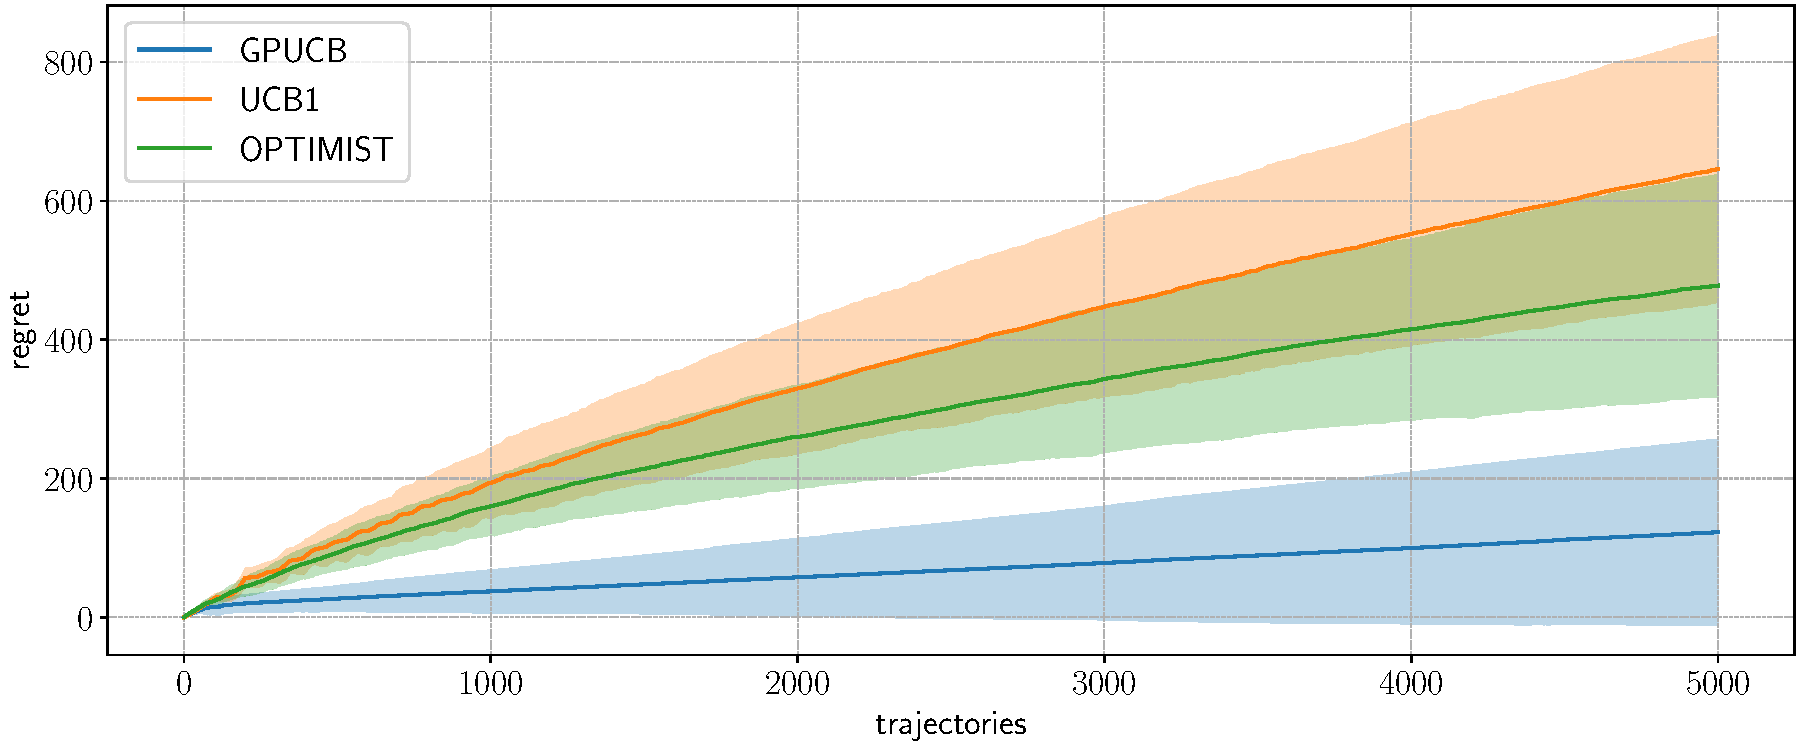
\includegraphics[width=\textwidth,height=\textheight,keepaspectratio]{Images/LQGcomparisonVar.pdf}
\caption{Cumulative regret in
the \gls{LQG} experiment, comparing
\gls{OPTIMIST}, \gls{UCB}1 and \gls{GPUCB} when learning both the mean and the standard deviation hyperparameters only.
(30 runs, 95\% c.i.)} 
\label{fig:LQGcomparisonVar} 
\end{figure*}

%%%%%%%%%%%%%%%%%%%%%%%%%%%%%%%%%%%%%%%%%%%%%%%%%%%%%%%%%%%%%%%%%%%%%%%%%%%%%%%%%%%%%%%%%%%%%%%%%%%%%%%%%%%%%%%%%%%%%%%%%%%%%%%%%%%

\section{Continuous Mountain Car}

\begin{figure*}[t!] 
\centering
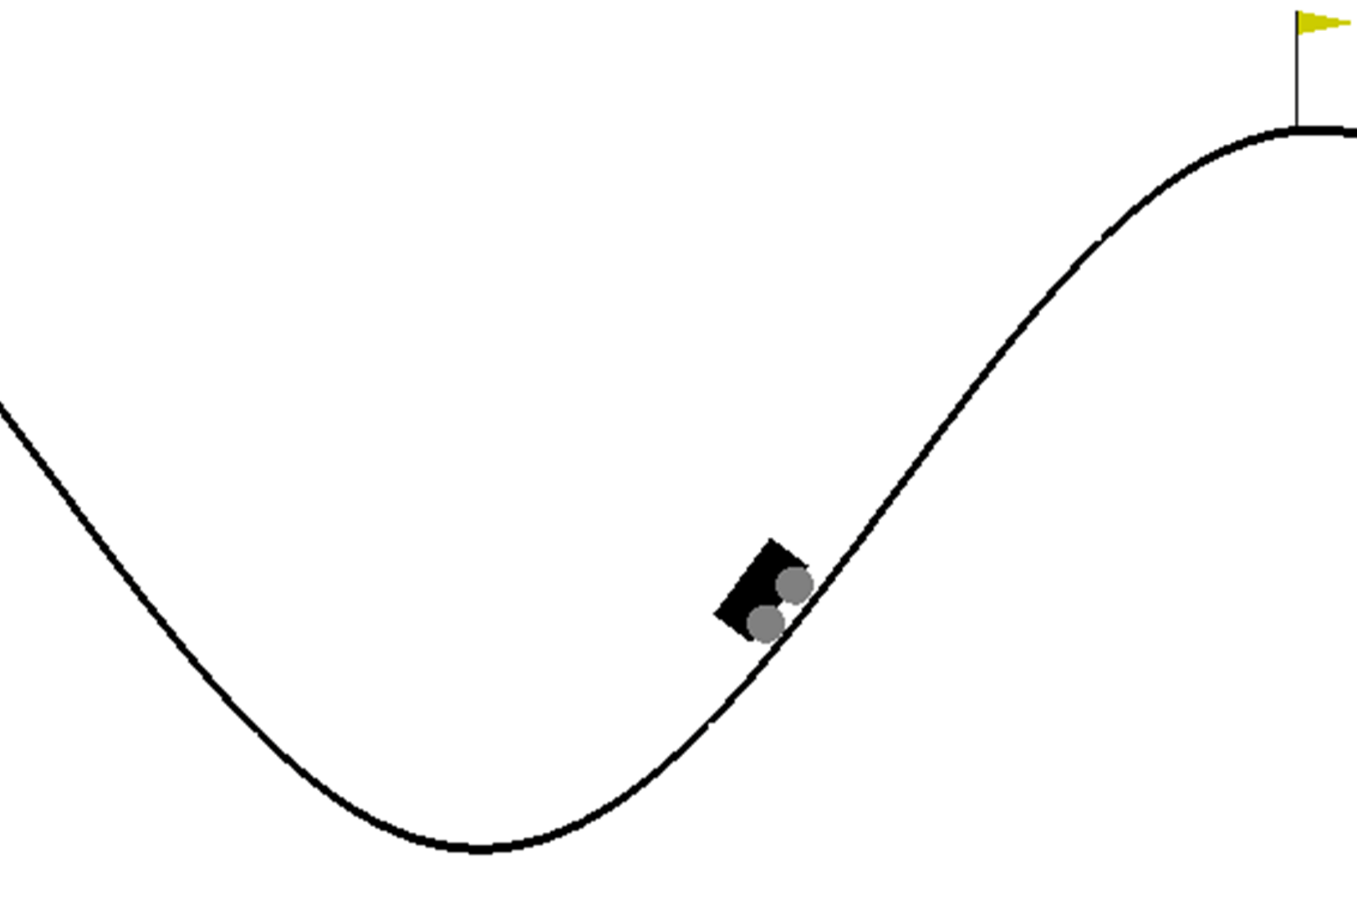
\includegraphics[width=.6\textwidth,keepaspectratio]{Images/MC.png}
\caption{Graphical representation of the Mountain Car problem.} 
\label{fig:MC}
\end{figure*} 

\begin{table}[t!]
\centering
\begin{tabular}{ccc|cc} 
\toprule
$\gamma$ & H & T & $\delta$ & k\\ 
\midrule
1.00 & 500 & 5000 & 0.20 & 3\\
\bottomrule
\end{tabular}
\caption{Task parameters (left side) and \gls{OPTIMIST} input parameters (right side) for the Continuous Mountain Car experiment.}
\label{tab:MCcoeff}
\end{table}

\begin{figure*}[t!] 
\centering
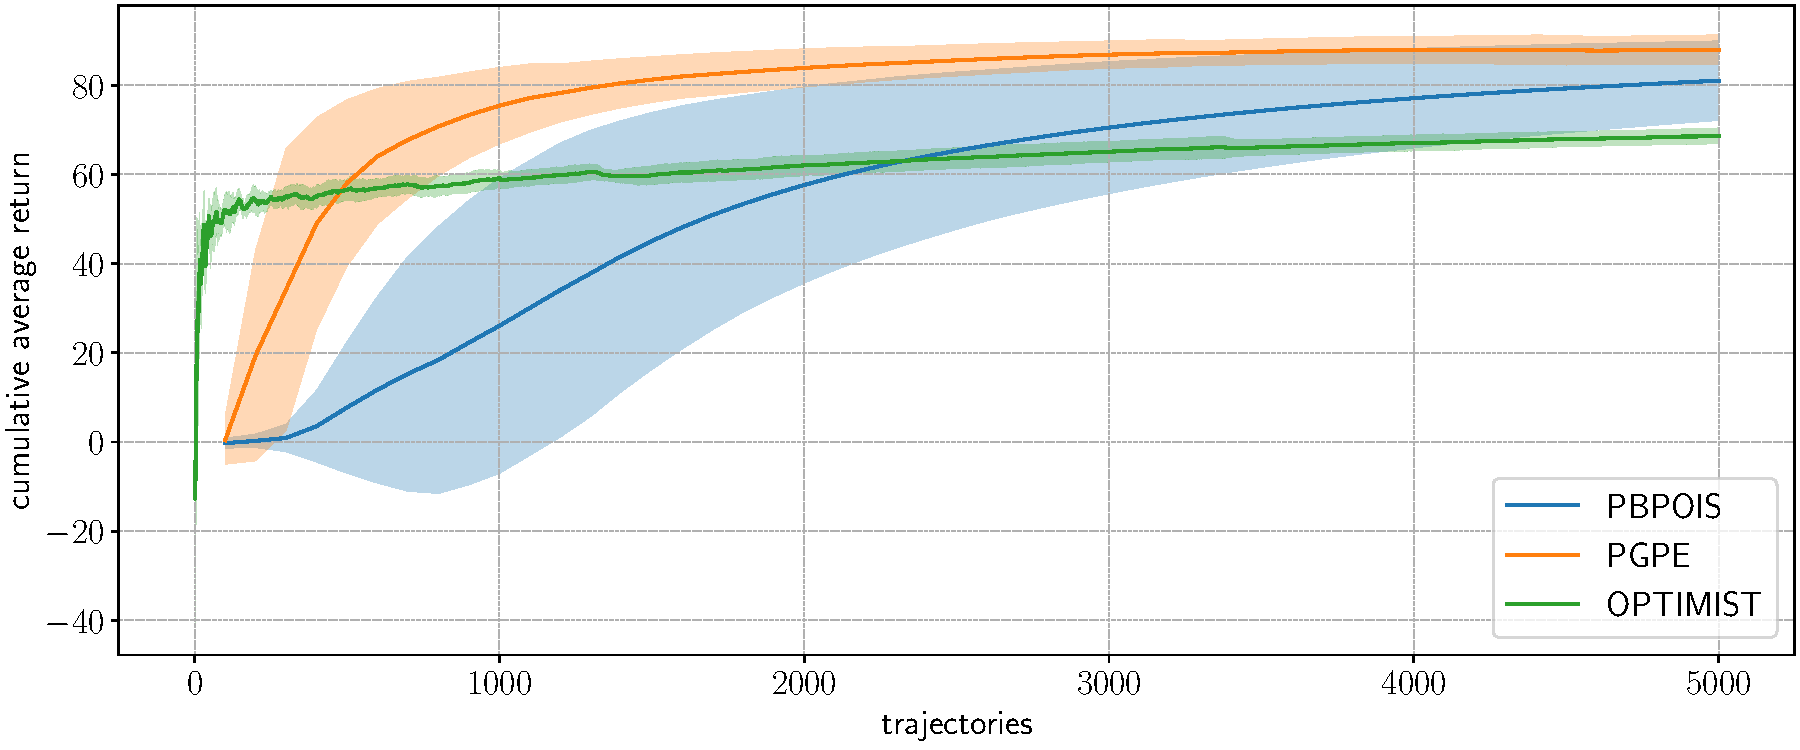
\includegraphics[width=\textwidth,height=\textheight,keepaspectratio]{Images/MC_mu.pdf}
\caption{Cumulative regret in
the \gls{LQG} experiment. Comparison between
\gls{OPTIMIST}, \gls{UCB}1 and \gls{GPUCB} when learning both hyperpolicy mean and the standard deviation.
(30 runs, 95\% c.i.)} 
\label{fig:MCcomparison} 
\end{figure*}

The second experiment, illustrates the behaviour of \gls{OPTIMIST}2  
when the parameters of the hyperpolicy belong to a compact (continuous) space, on the Continuous Mountain Car task\cite{brockman2016openai}. We chose the Continuous Mountain Car because it is a simple, well known, continuous problem and because it constitutes a relevant exploration challenge \wrt other simple tasks s.a. \gls{LQG}. 

In this problem, graphically represented in Figure (\ref{fig:MC}), the agent has to control the engine of an under-powered car in order to reach a target. The target is on top of a hill on the right-hand side of the car. If the car reaches it or goes beyond, the episode terminates. On the left-hand side, there is another hill. Climbing this hill can be used to gain potential energy and accelerate towards the target. On top of this second hill, the car cannot go further than a position equal to -1, as if there was a wall. Reward is 100 for reaching the target of the hill on the right hand side, minus the squared sum of actions from start to goal. This reward function raises an exploration challenge, because if the agent does not reach the target soon enough, it will figure out that it is better not to move, and won't find the target eventually. The state space $\Sspace=[-1.20,0.60]\times[-0.07,0.07]$ is constituted by a bi-dimensional vector with current position and velocity of the car. The action space $\Aspace\in\Reals$ is continuous: positive values correspond to a forward engine traction, negative values to backward engine traction. Every episode starts with the car in a random position between $-0.6$ and $-0.4$, with null velocity. The agent samples $H=500$ steps-long trajectories with a discount factor of $\gamma=1.00$ (the rationale of this choice is discussed in Remark (\ref{rk:undiscounted})), for a total of $T=5000$ iterations. 

In our experiments we use a Gaussian hyperpolicy with a two-dimensional learnable mean $\vmu=\vxi=(\xi_1, \xi_2)^T$, within a box $\vmu\in[-1,-1]\times[0,20]$, and a fixed covariance $\Cov=\mathrm{diag}(0.15^2,3^2)$. Concerning the confidence and discretization schedules for \gls{OPTIMIST}2, we adopted those suggested in Theorem (\ref{th:regretdiscretized}), \ie ${\delta_t = \frac{6\delta}{\pi^2t^2\left(1+\left\lceil t^{\nicefrac{1}{\kappa}}\right\rceil^d\right)}}$ and $\tau_t=\lceil t^{\frac{1}{\kappa}} \rceil$, with $\delta=0.2$ and $k=3$. The choice of $k$ influences the granularity of the discretization. Since $\tau_t=\lceil t^{\frac{1}{\kappa}} \rceil$ the granularity is non-decreasing with time, but smaller values of $k$ allow for a finer granularity at a given iteration $t$. For more information about the choice of $k$, refer to Remark (\ref{rk:discretization}). The parameters used in the Mountain Car experiments are summarized in Table (\ref{tab:LQGcoeff}).

We compare \gls{OPTIMIST}2 (\ref{alg:2}) against parameter-based policy optimization algorithms \gls{PGPE} (\ref{alg:PGPE}) and \gls{PBPOIS} \cite{metelli2018policy}. The latter is a parameter-based off-policy policy search algorithm which optimizes a lower bound of the performance estimator. Similarly to \gls{OPTIMIST}, this estimator is built upon single importance sampling. We chose to compare \gls{OPTIMIST} with \gls{PBPOIS} not only because of this similarity, but also because of their intrinsic difference. In fact, despite being both off-policy algorithms based on importance sampling, \gls{PBPOIS} optimizes a lower bound on the performance, which implies a very limited exploration. By contrast, \gls{OPTIMIST} optimizes an upper bound on performance, accordingly to the \gls{OFU} principle. \gls{OPTIMIST} and \gls{PBPOIS} are also compared with \gls{PGPE}, which laid the foundations for both of them. Moreover, \gls{PGPE} too is known to lack exploration of the parameter space. Finally, note that, unlike \gls{OPTIMIST}, both \gls{PGPE} and \gls{PBPOIS} adopts natural policy gradient ascent to optimize their hyperpolicies.
The best learning rate $\alpha$ for \gls{PGPE} was searched in the set $\{3, 2, 1, 0.1, 0.01, 0.001\}$. For \gls{PBPOIS}, we used the suggested hyperparameters. \\

Results are shown in Figure (\ref{fig:MCcomparison}). We can notice that \gls{OPTIMIST}2 is able to learn a good policy in a very short time thanks to its better exploration capabilities. However, the policy gradient methods outperform it on the long run. In fact, the exploitative behaviour of the other two algorithms make them more performant \wrt \gls{OPTIMIST}, which continue to explore even after having found suitable parameters in few iterations. Even though these results might not be satisfactory from a performance point of view, our primary goal was to develop a \gls{PS} algorithm that would explore effectively the space of parameters. From this point of view, the results turn out to be successful. To convince ourselves of this claim, we refer to Figure (\ref{fig:MCgain}), in which we show the density estimation of the probability distribution induced over the arm set $\vxi=\vmu$ by \gls{PGPE} (left) and \gls{OPTIMIST} (right). The estimation has been carried out by means of the Gaussian kernel density estimator \cite{scott2015multivariate} implemented in the SciPy library.\footnote{https://docs.scipy.org/doc/} Intuitively, this represents the likelihood of each two-dimensional arm to be pulled by either \gls{PGPE} or \gls{OPTIMIST}. 

\begin{figure*}[t!] 
\centering
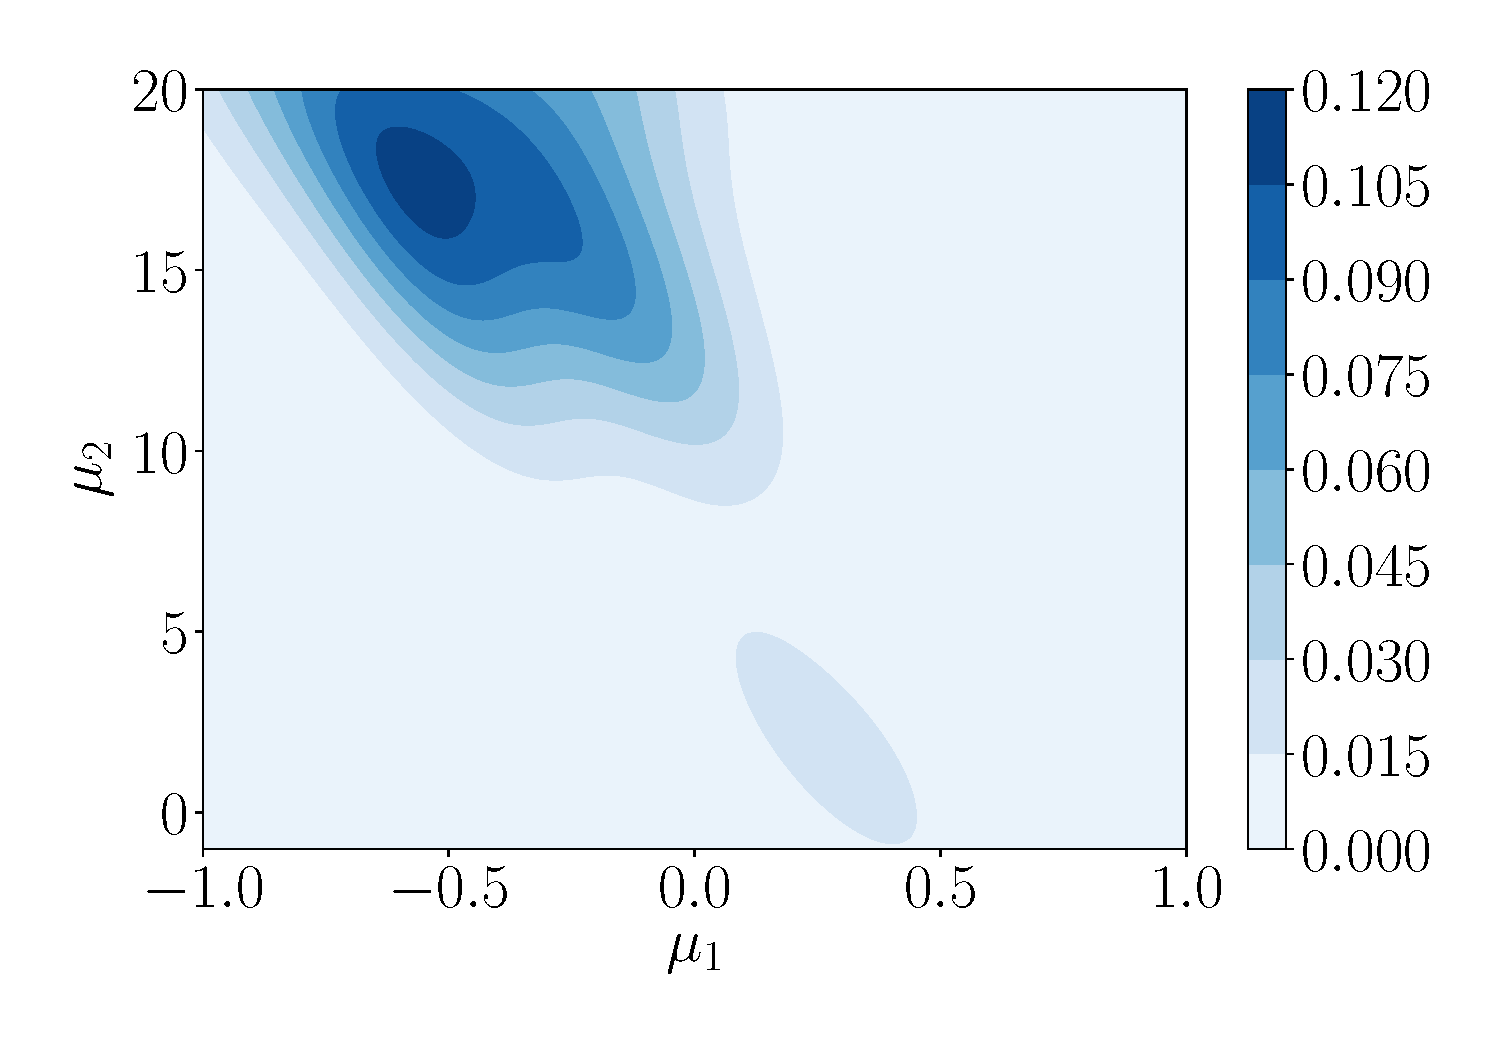
\includegraphics[width=.5\textwidth]{Images/MCgainPGPE.pdf}\hfill
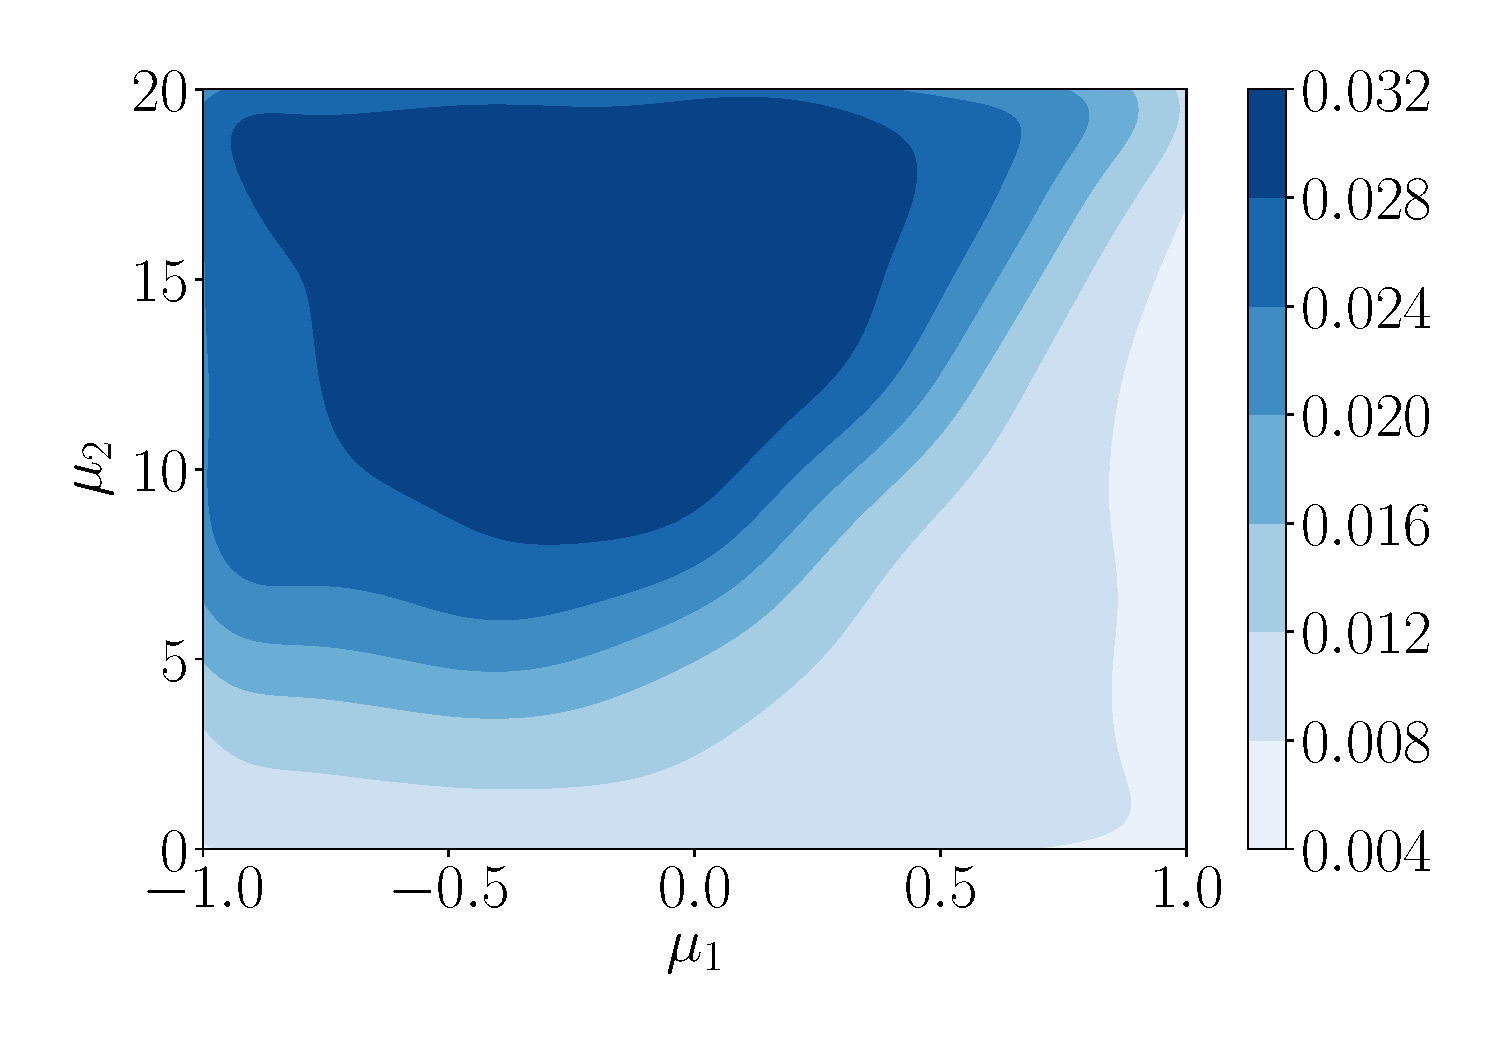
\includegraphics[width=.5\textwidth]{Images/MCgainOPTIMIST.pdf}
\caption{Gaussian kernel density estimation \cite{scott2015multivariate} of the probability distribution of the arm set $\vxi=\vmu$ induced by \gls{PGPE} (left) and \gls{OPTIMIST} (right).} 
\label{fig:MCgain}
\end{figure*} 

\begin{table}[t!]
\centering
\begin{tabular}{c|ccccc} 
\toprule
State-space dimension & $k=2$ & $k=3$ & $k=4$ & $k=5$ & $k=6$\\
\midrule
%$d=1$ & 71 & 18 & 9 & 6 & 5\\
$d=2$ & 5041 & 324 & 81 & 36 & 25\\
%$d=3$ & 357911 & 5832 & 729 & 216 & 125\\
$d=4$ & 2541168 & 104976 & 6561 & 1296 & 625\\
\bottomrule
\end{tabular}
\caption{Task parameters (left side) and \gls{OPTIMIST} input parameters (right side) for the Mountain Car experiment.}
\label{tab:granularity}
\end{table}

\begin{remark} \label{rk:undiscounted}
The rationale behind the choice of undiscounted ($\gamma=1.00$) rewards lies in the design of the reward system of the Continuous Mountain Car task. During learning, the car usually do not manage to reach the target before a few hundred iterations, while collecting rewards equal to minus the squared sum of actions in all previous steps. In such scenario, the agent would barely distinguish between a successful episode (that ended by reaching the target) and an unsuccessful one. For the sake of clarity, we will illustrate this situation with an example. Say that, after driving up and down the hills for 300 episodes, the agent finally manages to reach the target. Also, imagine that we are slightly discounting rewards with $\gamma=0.99$. In this situation, the positive reward received would be $r_{301}=0.99^{300}\cdot 100.00=4.90$, while the negative reward cumulated in previous steps ($h=1,2,\dots,299$) would at least be numbered in tens. This means that the return of the episode would still be negative and numbered in tens, because $|r_{301}|\ll |\sum_{h=0}^{299}\gamma^hr_{h+1}|$. Hence, the agent would not learn from this successful episode, because it could not tell it from an unsuccessful episode. This problem is solved by setting $\gamma=1$.
\end{remark}

\begin{remark} \label{rk:discretization}
Considering that \gls{OPTIMIST} needs to evaluate bound (\ref{eq:optimistindex}) for every arm, at each iteration, the finer the discretization schedule the longer the time required by numerical simulation. Indeed, the optimization of the bound is much more computationally demanding than any other operation undertaken by \gls{OPTIMIST}. In Table (\ref{tab:granularity}) we report the total number of arms resulting from different choices of $k$, according to the state-space dimension $d$, at final time step $T=5000$. As a reference, with the computing capacity at our disposal during this thesis project, the time needed for optimizing the bound over 5000 iterations was:

\begin{itemize}
\item approximately 4 hours with $d=2$ and $k=3$;
\item approximately 39 hours with $d=4$ and $k=4$.
\end{itemize} 

Evidently, our limited time and computing capacity did not allow for the finest of the discretization schedules. However, we think that the discretization adopted in the Mountain Car and Inverted Pendulum (discussed next) experiments was appropriate to the task at hand.
\end{remark}

%%%%%%%%%%%%%%%%%%%%%%%%%%%%%%%%%%%%%%%%%%%%%%%%%%%%%%%%%%%%%%%%%%%%%%%%%%%%%%%%%%%%%%%%%%%%%%%%%%%%%%%%%%%%%%%%%%%%%%%%%%%%%%%%%%%

\section{Inverted Pendulum}

\begin{figure*}[t!] 
\centering
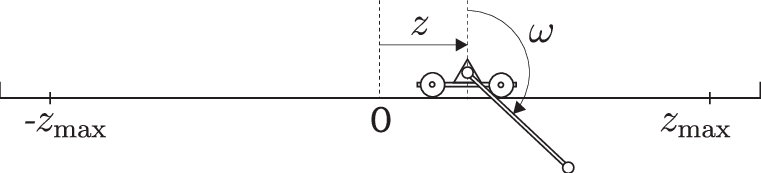
\includegraphics[width=.8\textwidth,keepaspectratio]{Images/inverted_pendulum.png}
\caption{Graphical representation of the Inverted Pendulum task.} 
\label{fig:invpend}
\end{figure*} 

\begin{table}
\centering
\begin{tabular}{ccc|cc} 
\toprule
$\gamma$ & H & T & $\delta$ & k\\ 
\midrule
0.99 & 500 & 10000 & 0.20 & 5\\
\bottomrule
\end{tabular}
\caption{Task parameters (left side) and \gls{OPTIMIST} input parameters (right side) for the Inverted Pendulum experiment.}
\label{tab:IPcoeff}
\end{table}

As third comparative experiment, we attempted to run \gls{OPTIMIST} on the Cart-Pole Swing-Up task \cite{tornio2006variational}, also referred to as Inverted Pendulum task. Unfortunately, in this case optimist was not able to learn any performant policy, neither optimal nor near-optimal. However, we present the experiment and some considerations on what could have gone wrong as a starting point for future developments.
This problem is a classic benchmark for non-linear control, which requires a thorough exploration for finding the optimal policy. The system consists of a pole attached to a cart, depicted in Figure \ref{fig:invpend}). The force applied to the cart can be controlled, and the goal is to swing the pole to an  upward  position  and  stabilise  it.  This  must  be accomplished without the cart crashing into the walls of the track. The state space $\Sspace\in\Reals^4$ consists of four observed variables. The position of the cart $u$ (constrained in $[-3,3]$), the angle  of  the  pole  measured  from  the upward  position $\phi$,  and  their  first  derivatives $u'$ and $\phi'$.  Control input is the force applied to the cart. The reward system is designed in a way that the agent receives a non-positive reward except when it manages to achieve an upward position:

\begin{equation}
\Rew(\boldsymbol{a}_t|\boldsymbol{s}_t)= \begin{cases}-100, &\text{if $|u_t|>3$} \\ \cos(\phi) &\text{if $|u_t|\leq3$} \end{cases}
\end{equation}

This task is known for requiring a thorough exploration of the parameter space because it is easy to encounter local optima which are far from the global optimum in terms of performance. An example would be a policy that continuously rotates the pole in order to receive a close-to-zero return, spending half of the time downwards and half upwards. The detailed dynamics and constraints for the simulated cart-pole system can be found in \cite{kimura1999efficient}, while for the implementation details (including the bounds applied to the position and the force) the reader can refer to the \emph{rllab} implementation\footnote{https://github.com/rll/rllab}. Before every trajectory, the system is initialized to a random state taken from the uniform distributions $u\in[-1,1]$, $u'\in[-2,2]$, $\phi\in[\pi-1,\pi+1]$, $\phi'\in[-3,+3]$. The agent samples $H=500$ steps-long trajectories with a discount factor of $\gamma=0.99$, for a total of $T=1000$ iterations.

In our experiments we used a Gaussian hyperpolicy with a four-dimensional learnable mean $\vmu=\{\mu_1, \mu_2, \mu_3, \mu_4\}$, within a box $\vmu\in[-0.2,0.2]^4$, and a fixed covariance $\Cov=\sigma^2\boldsymbol{I}$, with $\sigma=0.001$. Concerning the confidence and discretization schedules for \gls{OPTIMIST}2, we adopted those suggested in Theorem (\ref{th:regretdiscretized}), \ie ${\delta_t = \frac{6\delta}{\pi^2t^2\left(1+\left\lceil t^{\nicefrac{1}{\kappa}}\right\rceil^d\right)}}$ and $\tau_t=\lceil t^{\frac{1}{\kappa}} \rceil$, with $\delta=0.2$ and $k=4$. The summary of the parameters used in the Inverted Pendulum experiments is2 reported in Table (\ref{tab:IPcoeff}).

Unfortunately, \gls{OPTIMIST}2 failed to learn a good policy in this task.  Indeed, it failed to learn anything at all. This is clearly visible by looking at the hyperparameters curve over decision epochs: even after 10000 iterations the algorithm is still exploring (more or less) uniformly the parameter space. We report the curve of $\mu_1$ in Figure (\ref{fig:IPmu1}). The reason for this behaviour is likely to be $\sigma$. Indeed, for very small values of sigma, s.a. $\sigma=0.001$, the behavioural hyperpolicies adopted during learning do not share information with the target hyperpolicy. In other words, the \Renyi between the target and the mixture of behaviourals becomes very large and dominates the \gls{OPTIMIST} bound (\ref{eq:optimistindex}). We report the bound here for the sake of clarity:

\begin{align}
	&B_t^{1}(\vx,\delta_t) \coloneqq 
	\wc{\mu}_t(\vx)+\norm[\infty]{f}\left(\sqrt{2}+\frac{4}{3}\right)\left(\frac{d_{2}(p_{\vx_t}\|\Phi_{t})\log\frac{1}{\delta_t}}{t}\right)^{\frac{1}{2}}.
\end{align}

Evidently, when the \Renyi divergence is very high the second half (the \emph{exploration bonus}) dominates the bound, and obliges the agent to explore disregarding the estimated performances of the arms. This intuition is confirmed by looking at the very irregular plots of the truncated \gls{MIS} estimator $\wc{\mu}_t(\vx_t)$ and the exploration bonus $\norm[\infty]{f}\left(\sqrt{2}+\frac{4}{3}\right)\left(\frac{d_{2}(p_{\vx_t}\|\Phi_{t})\log\frac{1}{\delta_t}}{t}\right)^{\frac{1}{2}}$ for the arms $\vx_t$ selected at iterations $t=1,2,\dots,T$, reported in Figure (\ref{fig:IPbound}). The bonus (whose value is frequently over 10000) largely dominates the performance estimator (whose value is mostly negative). The intuitive counter-measure would be to adopt bigger values of $\sigma$. Unfortunately, the Inverted Pendulum has a very narrow set of near optimal arms and higher variances hinder learning, as confirmed by our numerical simulations. Indeed, this knot could represent another interesting starting point for further developments.

\begin{figure*}[t!] 
\centering
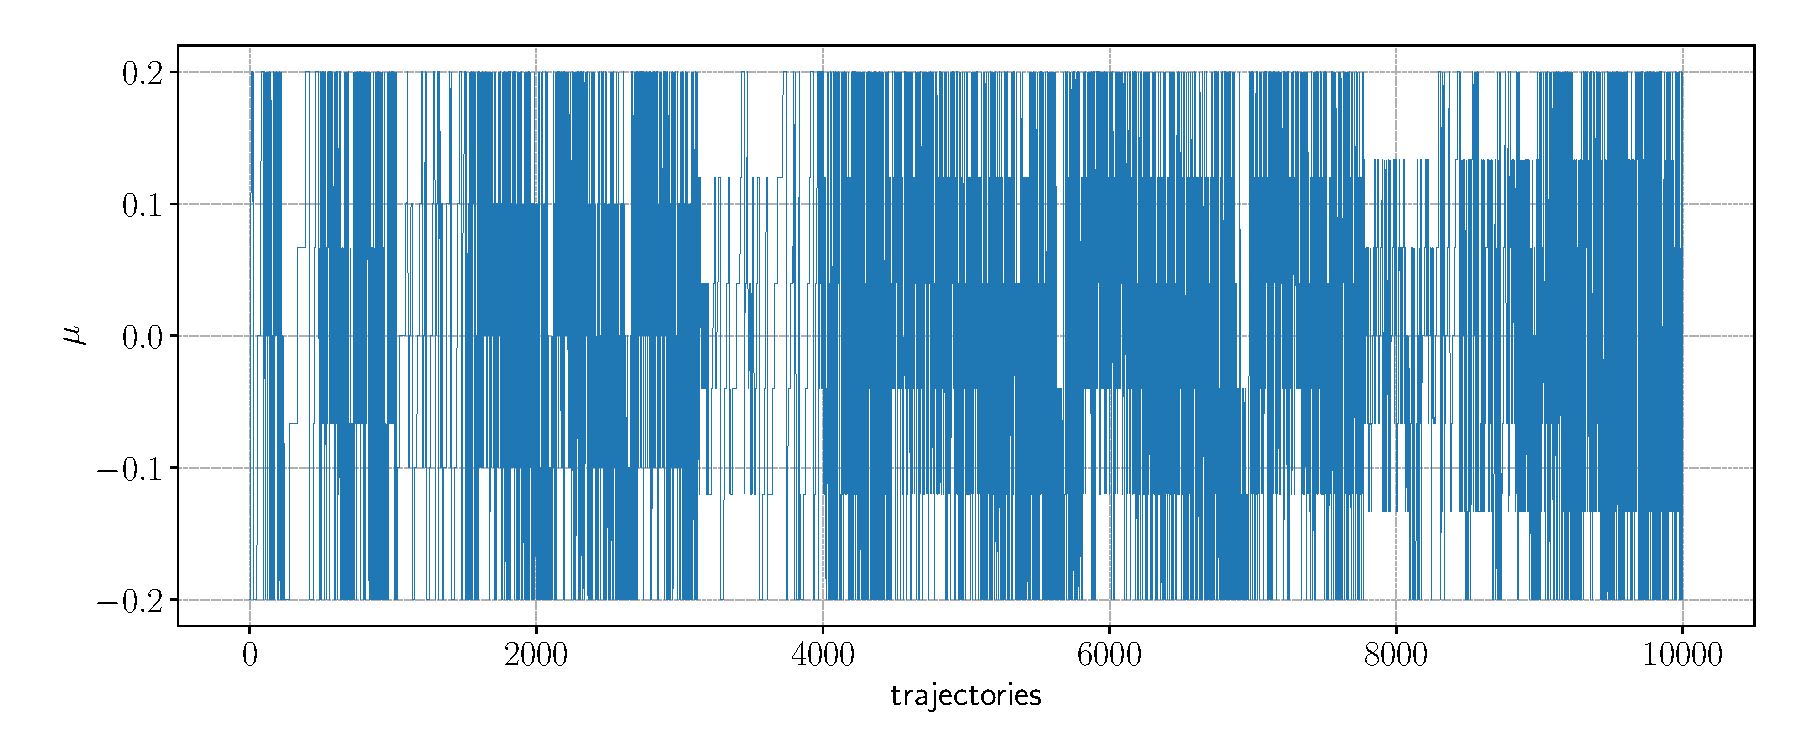
\includegraphics[width=\textwidth,keepaspectratio]{Images/IP_mu_1.pdf}
\caption{The hyperpolicy mean parameter selected at each iteration of \gls{OPTIMIST} in the Inverted Pendulum experiment.} 
\label{fig:IPmu1}
\end{figure*}

\begin{figure*}[t!] 
\centering
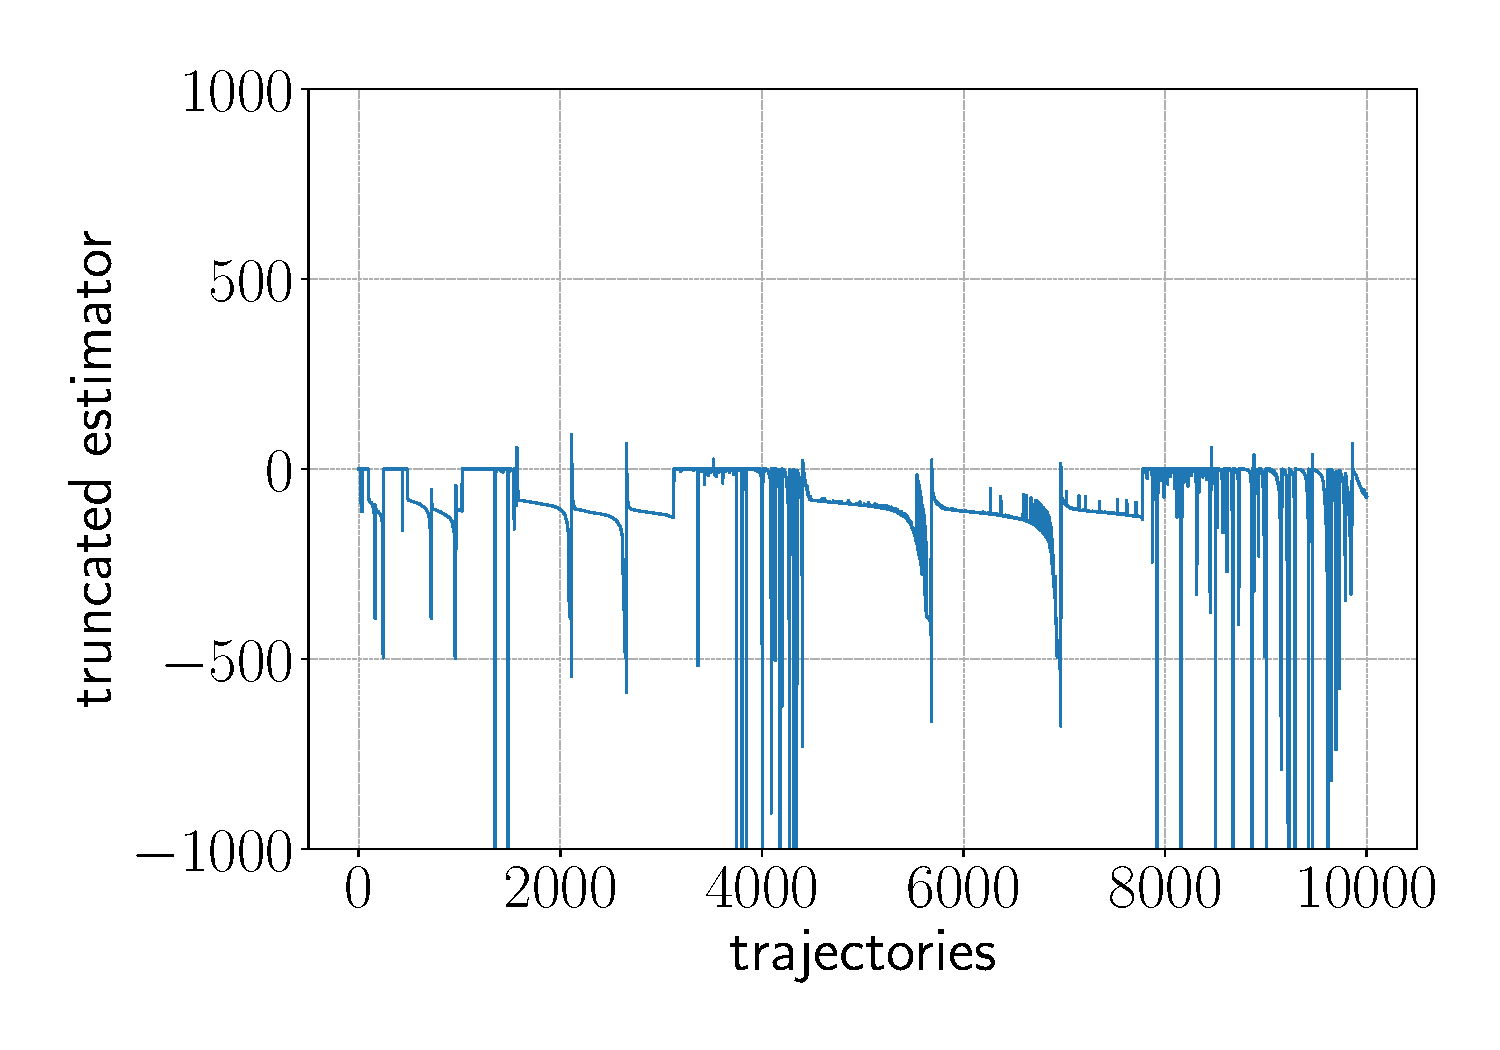
\includegraphics[width=.5\textwidth]{Images/IPmise.pdf}\hfill
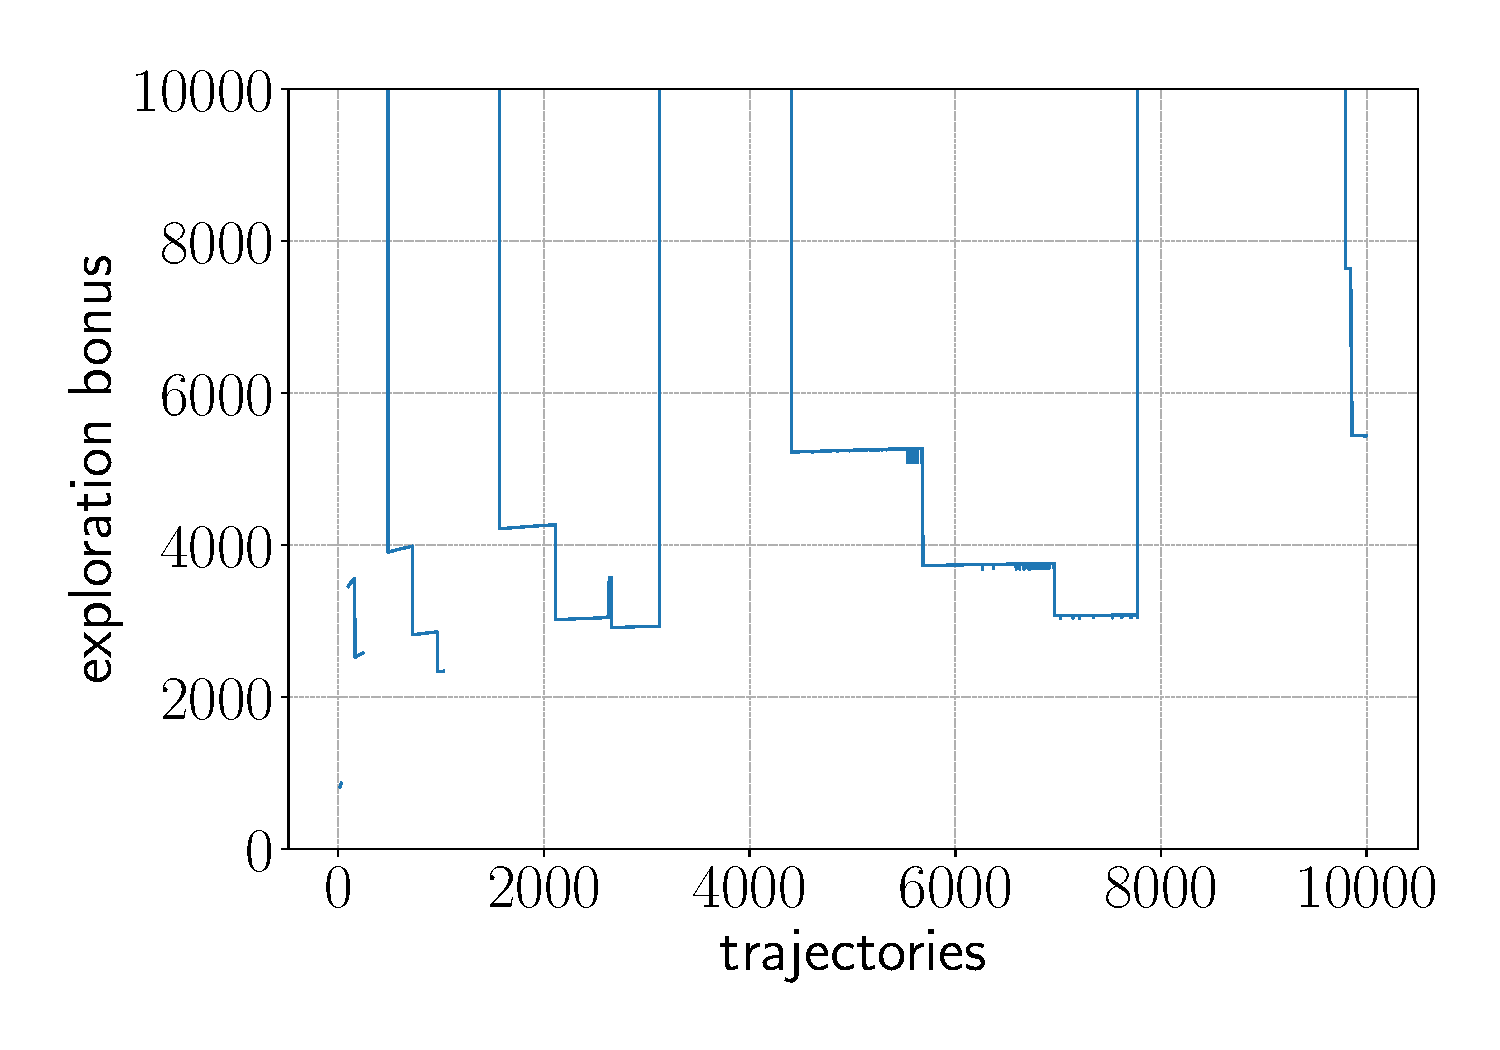
\includegraphics[width=.5\textwidth]{Images/IPbonus.pdf}
\caption{Truncated \gls{MIS} estimator (left) and exploration bonus (right) of the arms selected by \gls{OPTIMIST} at each iteration of the Inverted Pendulum experiment.} 
\label{fig:IPbound}
\end{figure*} 

%%%%%%%%%%%%%%%%%%%%%%%%%%%%%%%%%%%%%%%%%%%%%%%%%%%%%%%%%%%%%%%%%%%%%%%%%%%%%%%%%%%%%%%%%%%%%%%%%%%%%%%%%%%%%%%%%%%%%%%%%%%%%%%%%%%

\section{Action-based setting}

The reader may wonder why we did not carry out numerical simulations in the \emph{action-based} setting. Actually, we did make some experiments, but we briefly understood that there was a major obstacle represented by the computation of the \Renyi divergence. In fact, although what has been discussed in Section (\ref{sec:practical}) also applies to policies (not only hyperpolicies), the loss function can not be directly optimized since computing $d_{1+\epsilon}(p_{\vx}\|\Phi_t)$ requires the approximation of an integral over the trajectory space and, for stochastic environments, to know the transition model $\Tran$, which is unknown in a model free setting. For the sake of clarity, we report here the definition of the \Renyi divergence between the distributions $p_{\vtheta'}(\tau)$ and $p_{\vtheta}(\tau)$, induced over trajectories $\tau\in\Tau$ by the target $\pi_{\vtheta'}$ and behavioural $\pi_{\vtheta}$: \ref{eq:renyi}

\begin{align}
	d_{\alpha}(p_{\vtheta'}|p_{\vtheta}) = \left(\int_{\Tau}p_{\vtheta}(\tau)\left(\frac{p_{\vtheta'}(\tau)}{p_{\vtheta}(\tau)}\right)^{\alpha}\de \tau\right)^{\frac{1}{\alpha-1}}.
\end{align}

Simple bounds to this quantity, like $d_{\alpha}(p_{\vtheta'}|p_{\vtheta})\leq\sup_{s\in\Sspace}d_{\alpha}(\pi_{\vtheta'}(\cdot|s)|\pi_{\vtheta}(\cdot|s))^H$, besides being hard to compute due to the presence of the supremum, are extremely conservative since the Rényi divergence is raised to the horizon $H$. In our experiments, we tested action-based \gls{OPTIMIST} over the \gls{LQG} problem by estimating the exponentiated 2-\Renyi divergence between a proposal $Q$ and a target $P$ distribution as follows:

\begin{align} \label{eq:essrenyi}
\hat{d}_{2}(P|Q)=t / \wh{ESS}
\end{align}

where $t$ is the number of samples available, which in our case corresponds to the iteration step number, $w_{P/Q}$ is the importance weight, and $\wh{ESS}$ \cite{martino2017effective} is a well known estimator of the \emph{effective sample size} (ESS) \cite{kong1992note}, given by:

\begin{align}
\wh{ESS} = \frac{\norm[1]{w_{P/Q}}^2}{\norm[2]{w_{P/Q}}^2}
\end{align}

Ideed, the effective sample size is defined as \cite{kong1992note}

\begin{align}
ESS = \frac{t}{\Var_{x\sim Q}[w_{P/Q}(x)]+1}=\frac{t}{d_{2}(P|Q)}.
\end{align}

However, its estimator $\wh{ESS}$ is very rough and turned out to be useless in our case. The main problem of $\hat{d}_{2}(P|Q)$ (\ref{eq:essrenyi}) is that it is consistent with the true \Renyi divergence only for close enough target and behavioural policies ($P$ and $Q$). This means that the estimator does not allow to share the information obtained by a behavioural $Q$ with distant target distributions $P$. Moreover, by estimating the \Renyi from the samples we would lose \gls{OPTIMIST} theoretical guarantees on the regret. Therefore, this estimator proved to be impractical for the implementation of action-based \gls{OPTIMIST} and we decided to focus on the parameter-based setting. For future works, a study of a good estimator for the \Renyi would be another interesting starting point.